\documentclass[thesis.tex]{subfiles}

\chapter{Proposed Framework}
\section{BK.Synapse - A Framework for Distributed Neural Network Training}
In this section, we present a tool and framework for training neural networks in a distributed manner called BK.Synapse.

\subsection{Overview \& Motivation}
BK.Synapse provides a complete set of tools for training neural networks, including model and dataset managements, training configuration, monitoring and exporting results, combined with an intuitive, no-configuration distributed environment.

The use-cases and general design for BK.Synapse are inspired by NVIDIA DIGITS\footnote{\href{https://developer.nvidia.com/digits}{https://developer.nvidia.com/digits}} (Deep Learning GPU Training System). DIGITS' primary use case is training deep neural nets on multiple \glspl{gpu}, along with several computer vision-related utilities (eg. data visualization). The tool provides an user interface for interacting with and managing datasets, models, etc,... However, there are several downsides to DIGITS' design that motivated the creation of BK.Synapse, namely:
\begin{itemize}
    \item Despite supporting Caffe, TensorFlow and LuaTorch, DIGITS' workflow is heavily optimized for Caffe. This forces major rewrites and reconfiguration for non-Caffe frameworks. For example, TensorFlow models need to be fully written within a single file, while subclassing a parent class that makes testing quite difficult.
    \item DIGITS was designed for single-machine, local deployment. This means it can only utilize multiple \glspl{gpu} on the same machine, limiting scalability.
\end{itemize}

\begin{figure}[htp]
	\centering
	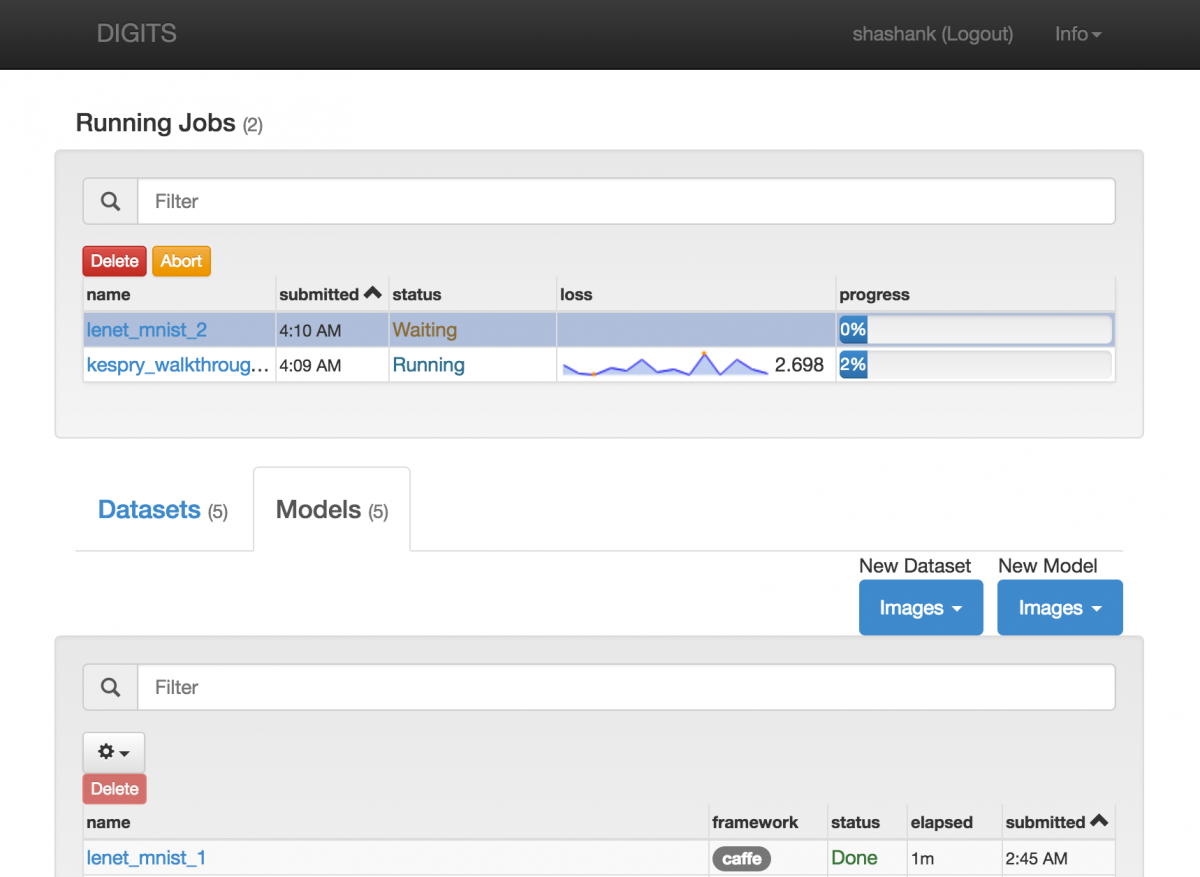
\includegraphics[width=\textwidth]{digits.png}
	\caption{An example of DIGITS' user interface}
	\label{fig:digits}
\end{figure}
\FloatBarrier

Due to these limitations, we aim to design BK.Synapse as a distributed training framework with little to no development overhead. Users should be able to train networks on multiple nodes with ease, while making minimal modifications to their existing codebases. With this in mind, we also target the more user-friendly PyTorch as the primary deep learning backend, with planned support for Keras and TensorFlow in the future. Table \ref{tab:digits_compare} shows a detailed comparison between BK.Synapse and DIGITS.

\begin{table}[]
\centering
\begin{tabu} to \textwidth {|l|X[c]|X[c]|}
    \hline
    \multicolumn{1}{|c|}{\textbf{Feature}} & \textbf{DIGITS} & \textbf{BK.Synapse} \\ \hline
    Single-node multi-GPU support & \cmark & \cmark \\ \hline
    Job monitoring \& management & \cmark & \cmark \\ \hline
    Open source & \cmark & \cmark \\ \hline
    Multiple node support & \xmark & \cmark \\ \hline
    Arbitrary models and datasets & \xmark & \cmark \\ \hline
    Data visualization & \cmark & \xmark \\ \hline
    Model visualization & \cmark & Partial (via \gls{tensorboard}) \\ \hline
    Backends & Caffe, TensorFlow, LuaTorch & PyTorch, Keras (planned), TensorFlow (planned) \\ \hline
\end{tabu}
\caption{Feature comparison between DIGITS and BK.Synapse}
\label{tab:digits_compare}
\end{table}

Aside from DIGITS, we also take note of other similar tools in the domain, namely DeepCognition\footnote{\href{https://deepcognition.ai/}{https://deepcognition.ai/}}, Google Colaboratory\footnote{\href{https://colab.research.google.com/}{https://colab.research.google.com/}}, etc,...

BK.Synapse is open source and hosted at \href{https://github.com/lanPN85/BK.Synapse}{https://github.com/lanPN85/BK.Synapse}.

We shall describe BK.Synapse's design and technical implementation in the following sections.

\subsection{Core Concepts}
There are 4 core concepts that define the user's workflow in BK.Synapse (Figure \ref{fig:workflow}):
\begin{enumerate}
    \item Datasets: A dataset is a collection of arbitrary files used for training (eg. images, text files,...). There is no pre-defined format, and users can simply compress their existing data and upload to the server.
    \item Models: A model contains the code for the user's custom network. In order to facilitate dynamic loading during runtime, this code needs to adhere to a simple interface that will be described in later sections.
    \item Data loaders: A data loader is the glue component that connects a dataset and a model. Conceptually, data loaders are the same as PyTorch's Dataset or Keras' Sequence. They define how data from datasets should be loaded and transformed in order to be fed into models.
    \item Jobs: A job puts the above components together to create a complete training pipeline. It also specifies many hyperparameters for training (eg. learning rate, batch size,...) and the nodes to be used for the training process.
\end{enumerate}

\begin{figure}[htp]
	\centering
	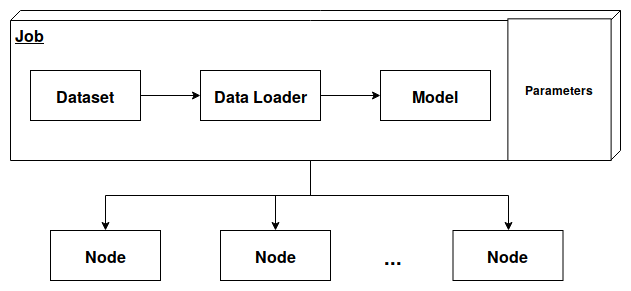
\includegraphics[width=0.6\textwidth]{workflow.png}
	\caption{BK.Synapse' core concepts and workflow}
	\label{fig:workflow}
\end{figure}
\FloatBarrier

\subsection{System Architecture}
At a high level, BK.Synapse consists of 4 primary components: the \gls{api} server, worker nodes, data store, and the web application (Figure \ref{fig:architecture}).

\begin{figure}[htp]
	\centering
	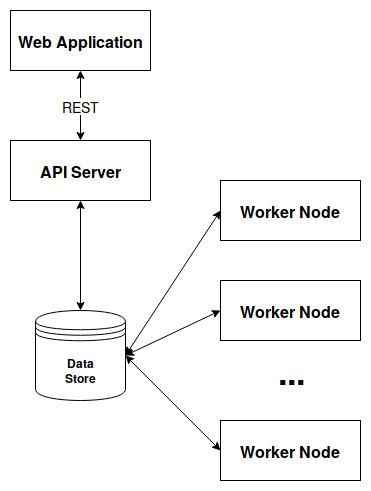
\includegraphics[width=0.5\textwidth]{architecture.png}
	\caption{BK.Synapse's high-level architecture}
	\label{fig:architecture}
\end{figure}

The system is designed in a client-server pattern, with loosely coupled components that can be deployed separately. The deployment environment should have high availability (ie. nodes should not fail or shutdown regularly) and trusted.

The API server exposes an application programming interface via HTTP \gls{rest}. Clients can use standard HTTP requests from any supported language to access the system. The server is implemented using the Flask \cite{Grinberg:2014:FWD:2621997} framework.

Worker nodes handle the bulk of calculations during training. Each node runs a background process called the node \gls{daemon}, collecting hardware status and notifying BK.Synapse of the node's availability.

The data store (or root folder) is used as the shared data space between the API server and worker nodes. It points to a folder that is accessible from all nodes within the system, and contains all user-uploaded data as well as additional metadata. Several mechanisms can be employed to create the data store, namely:
\begin{itemize}
    \item Using filesystem mount: The data store is created on one node, then mounted throughout the network using Linux's NFS or SMBD protocol. This provides good guarantees in terms of writes, however there may be overhead during training when data files need to be continually read.
    \item Using object store mount: Cloud object stores such as Amazon S3 or Minio provide utilities that allows mounting onto a folder. This can be significantly less trivial to setup compared to the first option, however it can perform much faster depending on the object store implementation.
\end{itemize}

The primary reason to use a native file folder as data store, as opposed to an object store or database is due to accessiblity. As stated, BK.Synapse aims to be simple and user-friendly, and thus should expose a simple folder structure to users instead of a complex data management system. With our setup, users can reuse their data loading logic directly into their BK.Synapse code.

Finally, the web application is a client that uses the BK.Synapse API, providing users with access to the system via a graphical interface (Figure \ref{fig:bks_example_1}). It also includes documentations and various examples of using BK.Synapse. The application is built using the Vue\footnote{\href{https://vuejs.org/}{https://vuejs.org/}} framework.

\begin{figure}[htp]
	\centering
	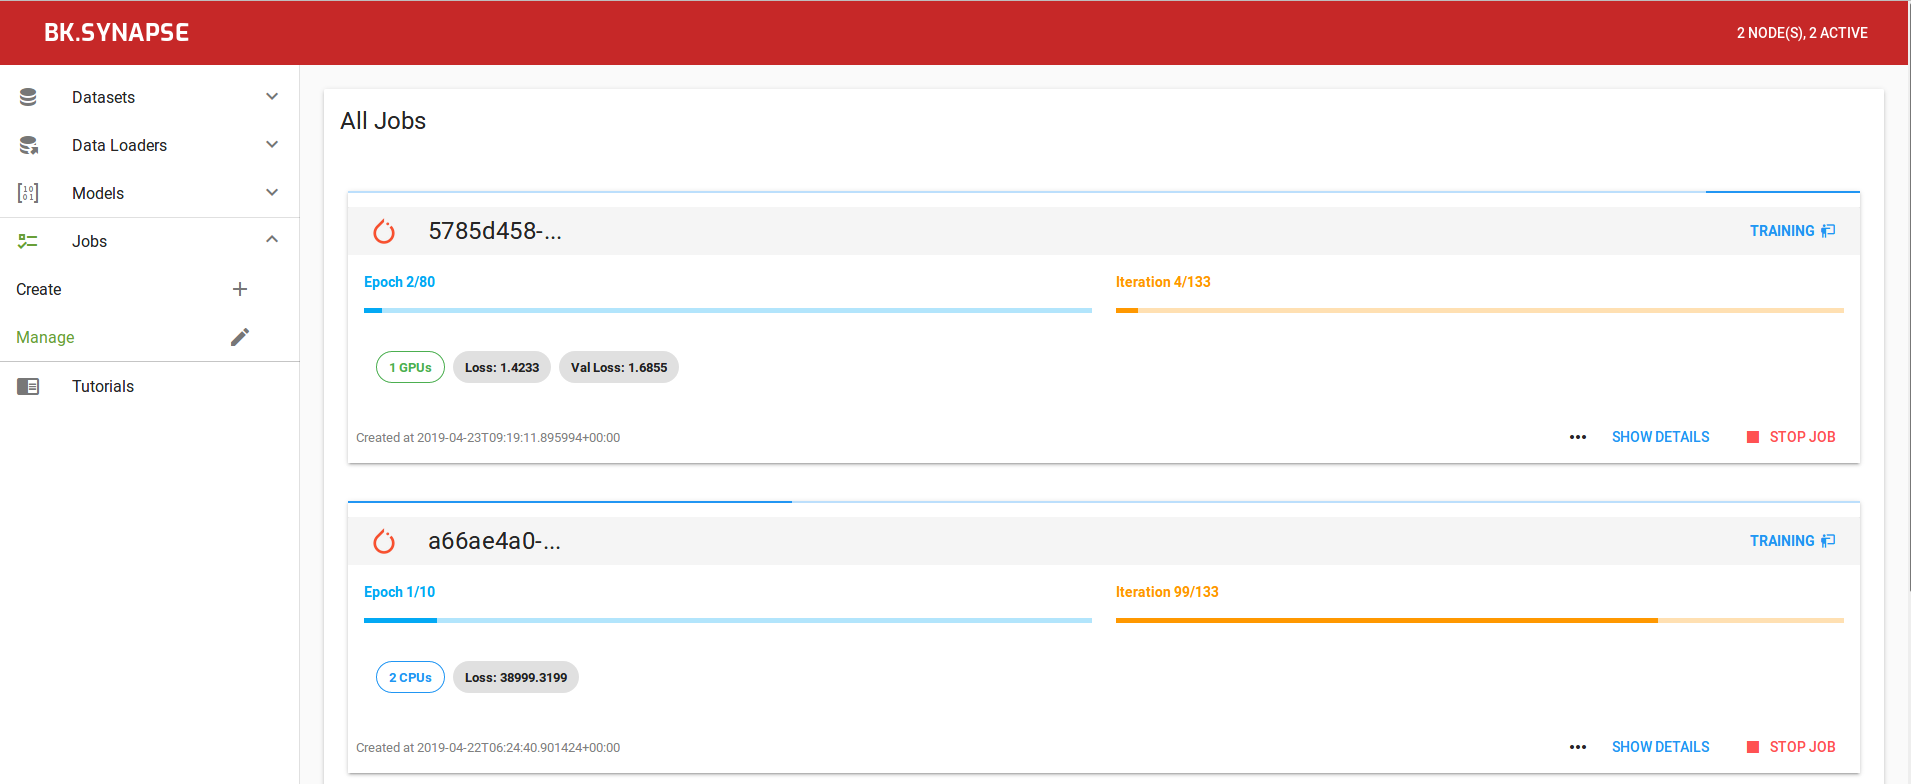
\includegraphics[width=\textwidth]{bks_example_1.png}
	\caption{The BK.Synapse web application}
	\label{fig:bks_example_1}
\end{figure}
\FloatBarrier

\subsection{Object Management Model}
BK.Synapse manages objects directly through the filesystem within the shared datastore. The directory structure is shown in Figure \ref{fig:bksynapse_tree}.

\begin{figure}[htp]
	\centering
	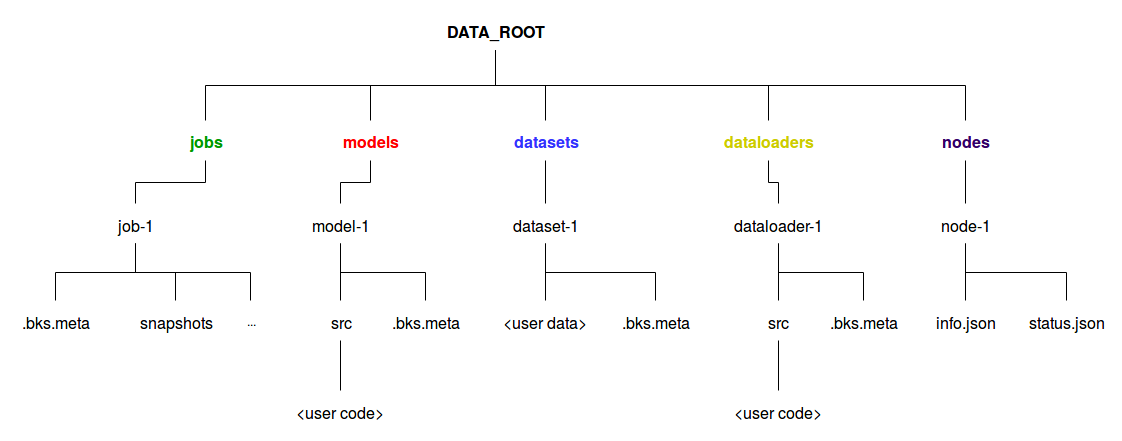
\includegraphics[width=\textwidth]{bksynapse_tree.png}
	\caption{The BK.Synapse directory structure}
	\label{fig:bksynapse_tree}
\end{figure}

Each object is assigned its own folder. Aside from nodes, whose metadata is provided by the node daemon in \lstinline{info.json}, every object stores metadata in \lstinline{.bks.meta}, a small JSON file that helps initialize these objects.

Models and data loaders store user-uploaded code in the \lstinline{src/} folder.

The API provides several standard operations on each object type, including get queries, update, create, and delete. For uploading code and data, the user is required to put all source files and folders into a zip file, which is decompressed on the API server into the datastore.

Even though a lot of metadata are stored as JSON documents, we chose not to use a full-fledged \gls{nosql} like MongoDB or a \gls{sql} like PostgreSQL. Our arguments for this decision include:
\begin{itemize}
    \item Consistency: since datasets, model code and loader code need to be placed in a datastore folder, it makes sense to store all data there as well, turning the datastore into a communication hub for the entire system. Using a database would introduce consistency constraints and require various checks and failure scenarios, while potentially slowing down overall performance.
    \item Simplicity: JSON files are easily read and accessed, which helps keep configuration to a minimum and eliminates complex database integration code. This also provides portability, as the entire system state can be easily packaged and replicated.
    \item Redundancy: With its current features, BK.Synapse would gain little from using databases. Most of our queries are simple get queries that might take even longer when put into databases. However, future improvements such as full-text search would compel us to use a database as a mirror to enable efficient queries.
    \item Finally, this decision is somewhat influenced by DIGITS, which uses a similar directory model to store jobs, albeit with a less portable file format (Pickle).
\end{itemize}

\subsection{User Code Execution}
The core BK.Synapse runtime is capable of embedding user-defined classes and functions across multiple files/packages into the training procedure. This requires the user to define entrypoints that the runtime can detect. These include:
\begin{itemize}
    \item A file named \lstinline{bks_model.py}, containing the class \lstinline{UserModel} to define a model. \lstinline{UserModel} must implement a \lstinline{loss()} method that defines the loss function used in training. Optionally, if a \lstinline{metrics()} method is defined, then it is used to calculate additional metrics (eg. accuracy). For PyTorch models, \lstinline{UserModel} must subclass \lstinline{Module}.
    \item A file named \lstinline{bks_dataset.py}, containing the class \lstinline{UserDataset} and (optionally) \lstinline{UserValDataset}, which define the loading logic for a data loader. PyTorch-compatible loaders need to subclass PyTorch's \lstinline{Dataset} class.
\end{itemize}

These interfaces are meant to wrap around existing code using inheritance, thus preserving their original behavior and facilitate testing, while still conforming to BK.Synapse's specifications. On the other hand, simpler models and loaders can simply be written directly into the given class.

\begin{lstlisting}[caption={An example UserModel wrapped around a simple CNN}]
import torch
import torch.nn as nn
import torch.nn.functional as F

class Net(nn.Module):
# ConvNet with 2 convolution blocks followed by dropout 
# and 2 fully connected layers
    def __init__(self):
        super(Net, self).__init__()
        self.conv1 = nn.Conv2d(1, 10, kernel_size=5)
        self.conv2 = nn.Conv2d(10, 20, kernel_size=5)
        self.conv2_drop = nn.Dropout2d()
        self.fc1 = nn.Linear(320, 50)
        self.fc2 = nn.Linear(50, 10)

    def forward(self, x):
        x = F.relu(F.max_pool2d(self.conv1(x), 2))
        x = F.relu(F.max_pool2d(self.conv2_drop(self.conv2(x)), 2))
        x = x.view(-1, 320)
        x = F.relu(self.fc1(x))
        x = F.dropout(x, training=self.training)
        x = self.fc2(x)
        return x

class UserModel(Net):
    def loss(self, output, target):
        return F.cross_entropy(output, target, reduction='mean')

    def metrics(self, output, target):
        preds = torch.argmax(output, dim=1)
        total = preds.shape[-1]
        correct = (preds == target).float()
        acc = torch.sum(correct) / total
        return {
            'accuracy': acc.item()
        }
\end{lstlisting}

The mechanics for embedding user code is relatively simple, and is partially based on DIGIT's method for loading TensorFlow models. We use Python's built-in \lstinline{exec()} function, which can execute a string as Python code within the current environment. A major difference in our implementation is allowing relative imports from within the model directory. Since actual projects would have their code split into multiple files, this is a critical feature to ensure ease of use. We accomplish this by manipulating \gls{py}'s path object (\lstinline{sys.path}). The Python path is a list of filesystem paths that informs the interpreter òf where to look for modules. By inserting the source code root path to Python's path, we can emulate the user's environment and allow relative package loading. Once the neccessary modules are loaded, the injected path is removed to avoid pollution and/or conflict (Figure \ref{fig:codeload}).

\begin{figure}[htp]
	\centering
	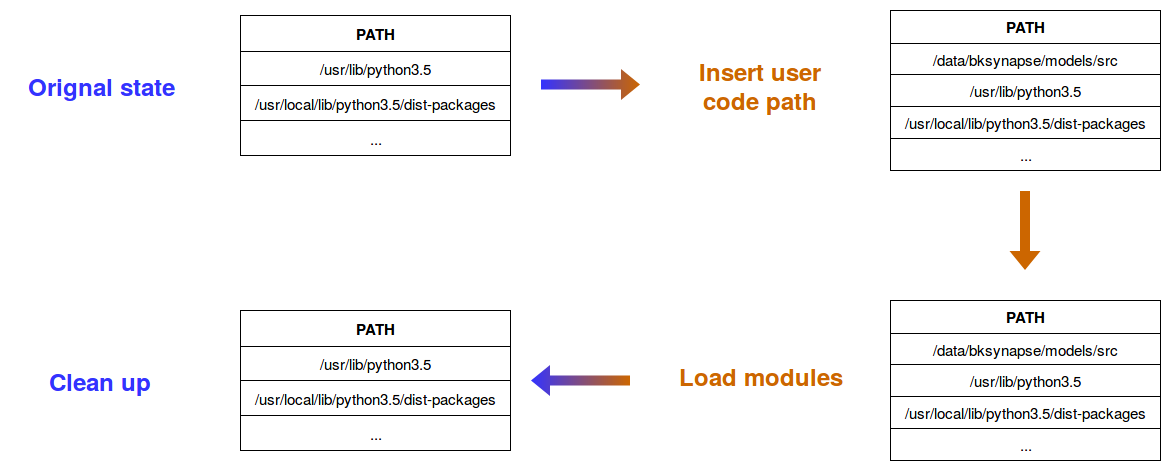
\includegraphics[width=0.95\textwidth]{codeload.png}
	\caption{Dynamic code loading procedure}
	\label{fig:codeload}
\end{figure}

\subsection{Parallelization Techniques}
BK.Synapse's key feature is being able to scale easily across multiple machines. The infrastructure layer supports this by keeping track of node IPs using node daemons, making it easy to add new nodes or detect failures. The actual parallel execution is implemented with Horovod \cite{DBLP:journals/corr/abs-1802-05799} and MPI \cite{Forum:1994:MMI:898758}.

Horovod provides a set of utilities to leverage MPI and associated acceleration methods (eg. NCCL) to perform multi-node training:
\begin{itemize}
    \item An \lstinline{hvd.rank()} function that provides the process MPI rank, as well as \lstinline{hvd.local_rank()} to query local MPI rank.
    \item A \lstinline{DistributedSampler} for PyTorch that partitions datasets into non-colliding sets for each process rank.
    \item A ring allreduce implementation (\lstinline{hvd.allreduce()}) providing efficient value aggregation.
    \item A \lstinline{DistributedOptimizer} wrapper for PyTorch that allows networks to be updated over multiple nodes.
\end{itemize}

The training script is invoked using \lstinline{mpirun}, from a subprocess spawned by the API server when the start endpoint is called. The server collects the selected worker nodes' IPs and generate a command as follow:
\begin{lstlisting}[language=Bash]
mpirun --allow-run-as-root -bind-to none -map-by slot\\
    -mca plm_rsh_args "-p 17992" -mca pml ob1 -mca btl ^openib\\
    -mca btl_tcp_if_include 192.168.1.0/24  -x LD_LIBRARY_PATH\\
    -x PATH -x BKSYN_DATA_ROOT -v -np 2\\
    -H 192.168.1.2:1,192.168.1.8:1\\
    python /usr/bin/bksynapse/pytorch/train.py\\
        --job-id d20db7d2-2f22-4f86-bbc7-8e93c5239132
\end{lstlisting}

A lot of configuration is handled by BK.Synapse to ensure proper MPI communication between nodes, in regards to the \lstinline{-mca} options above.

We make use of the rank 0 node as the logger, periodically writing the job's status to the shared folder. Interrupts are handled using a special lock file (\lstinline{job.lock}) that gets checked at regular intervals.

For nodes with multiple \glspl{gpu}, the default behavior is to use all those that are available, each getting its own MPI process. We use local rank to pin each process to its respective GPU.

\subsection{Monitoring Mechanisms}
The training script handles more than model training. In addition, it periodically logs progress information into a status update file (\lstinline{status.json}). Clients can query the corresponding job's endpoint to receive this file's contents, and be notified of the training process. Additionally, status updates are also appended to a \lstinline{history.toml} file, which serves as the job's history logs and used for future analytics. As job histories tend to be very long, we opt to store it as a TOML\footnote{\href{https://github.com/toml-lang/toml}{https://github.com/toml-lang/toml}} array instead of a JSON document. On top of being human readable, TOML arrays can be easily parsed as a file stream without loading the whole document, which immensely improves query speed.

\begin{lstlisting}[caption={An example history.toml file}, language=XML]
# ===Start===
[[entry]]
state = "SETUP"
isActive = true
epoch = 0
isStopped = false
totalIter = 0
timestamp = "2019-04-22T03:25:25.741491+00:00"
iter = 0
metrics = []
# ===End===

# ===Start===
[[entry]]
state = "TRAINING"
isActive = true
epoch = 0
isStopped = false
totalIter = 0
timestamp = "2019-04-22T03:25:36.699942+00:00"
message = "Starting training..."
iter = 0
metrics = []
# ===End===
\end{lstlisting}

The BK.Synapse web client polls the API backend every few seconds and updates the monitoring UI. Even though this is not as real-time as some other solutions (eg. WebSockets), we argue that there's no penalty for slightly slower progress updates. In addition, we find that the polling model creates a more consistent and stable interface to our system.

The training script also generates a TensorBoard log directory for further analysis, and handles saving checkpoints at regular intervals.

Similar to jobs, nodes are monitored using node daemons. A node daemon is deployed at each node, and is in fact a simple Python script that runs an infinite loop. Within the loop, the daemon i) queries CPU and GPU information, ii) updates the node status and iii) waits several seconds to the next loop. Constant information like GPU names, CPU frequency, etc... are collected on startup. Only status information, eg. RAM usage, GPU memory usage,... are constantly queried. This information is also polled and displayed by the BK.Synapse web app.

Each status update also contains a timestamp, used by the API server as a health check mechanism. If a node's timestamp is "stale" (i.e too far away from the current timestamp), that node is declared inactive.

\subsection{Deployment Model}
MPI requires a single port to be used for SSH connection across all machines. To avoid collision, we use the port 17992, and bind each container to the host machine's network stack.

For optimal performance, we have several deployment recommendations:
\begin{itemize}
    \item High-speed connections are preferred when setting up the node network(eg. InfiniBand). Note that this does not have to include the web server, since this is separate from the training runtime.
    \item Node \glspl{gpu} should have the same or similar capabilities. Otherwise, GPU speed or memory would be capped at the job's lowest-tier GPU, leading to wasted resources.
\end{itemize}

Our deployment workflow aims for simplicity and minimal configuration, allowing new nodes to be easily deployed. Using Docker containers helps isolate a lot of complex environment requirements, including SSH keys which are shared among nodes. Only a few system dependencies need to be setup, including:
\begin{itemize}
    \item GPU drivers: this component is shared in the NVIDIA-Docker runtime model, and needs to be installed for GPU nodes to function.
    \item Shared drive mount: the datastore mount method is deployment-specific, and needs to be manually configured.
    \item Networking configurations: several configurations related to network addressses have to be configured, as detecting correct configurations would be too unreliable. These values are mostly related to the IP address space, and can be trivially queried.
\end{itemize}

\subsection{Security Concerns}
In its current state, BK.Synapse should only be deployed in a trusted, private environment. This is due to a number of security concerns, including:
\begin{itemize}
    \item No access control or authorization has been implemented. This is however an important feature that will eventually be added once the API is more stable.
    \item The use of \lstinline{exec()} can create many attack vectors. Since \lstinline{exec()} would execute any Python command, a malicious agent can freely inspect or modify the system. Even though Docker provides some level of isolation, attackers can still easily cripple nodes or retrieve secret data. These vulnerabilities can be patched by setting up less-privileged users, or blocking certain modules from loading.
    \item MPI forces an open SSH port to be available on each node, which can be abused to grant full access to system nodes and datastore. This combined with the shared SSH keys bundled with the Docker container can pose a serious security risk.
\end{itemize}

Since this is somewhat out-of-scope, we will not go into detail on this topic. However, these problems will be addressed as the system moves toward public use.

\section{Comparison with DIGITS}
BK.Synapse is most similar in spirit to DIGITS, however we aim to improve on several perceived downsides.

BK.Synapse's key feature is distributed training, as opposed to single-node multi-GPU training in DIGITS. This allows our system to scale horizontally instead of vertically. At the same time, there's more complexity when deploying a distributed system. While DIGITS can be deployed from a single Docker container, it takes a lot more configuration to set up a BK.Synapse cluster.

Another point we aim to improve is reusing user code. While DIGITS is very streamlined for Caffe users, using TensorFlow or Torch code is difficult. BK.Synpase allows more freedom and flexibility for the user's code, creating a more efficient workflow.

We also try to improve on modularity, by separating the web frontend, API server and execution nodes. Although this incurs some additional complexity to communicate between these components, the modular design allows much more flexibility and aids further development.

\section{Case Study: RetinaNet for Text Region Detection}  \label{section:retinanet}
To fully evaluate BK.Synapse's effectiveness, we investigate its use in training RetinaNet, an existing CNN architecture for object detection.

RetinaNet \cite{Lin_2017} is a network architecture proposed by Lin et al in 2017. RetinaNet is a one-stage detector in similar spirit to YOLO, however it aims to match two-stage detectors in terms of accuracy while maintaining inference speed.

\subsection{Feature Pyramid Network}
RetinaNet improves primarily on Feature Pyramind Networks (FPN) \cite{Lin_2017_fpn}. FPN works on the intuition that it is better to take advantage of several feature maps (layer outputs) of a network for prediction, instead of just the final output. The reasoning for this is quite simple: smaller objects benefit from large, coarse feature maps where they are more visible, while larger/more complex objects are more easily detected in small, fine feature maps where they are more simplified. The network design is described in Figure \ref{fig:fpn}.

\begin{figure}[htp]
	\centering
	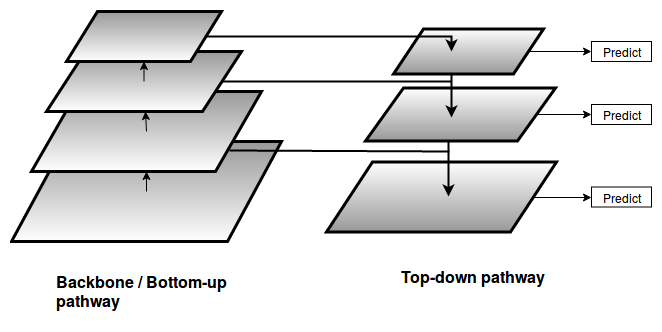
\includegraphics[width=\textwidth]{fpn.png}
	\caption{Feature Pyramid Network}
	\label{fig:fpn}
\end{figure}

FPN utilizes a secondary CNN architecture called the backbone. The backbone network can be any convolutional neural network, and is typically a commonly used architecture (eg. VGG, ResNet,...). The backbone's convolution blocks make up the bottom-up pathway, where feature maps of different layers are created. The authors define network "stages", in which convolution blocks have the same output size. In the case of ResNet, the authors used the activated output of each stage's residual block as feature maps.

A top-down pathway is used in conjunction with a conventional regressor/classifier pair. The final feature map is upsampled (using nearest neighbor upsampling) and added element-wise to the corresponding lower-level feature map from the bottom-up pathway. The bottom-up map undergoes 1x1 convolution to generate uniform channel dimensions, while the merged map also goes through a 3x3 convolution layer to reduce aliasing. This addition operation forms lateral connections, similar to UNet-type architectures. The resulting feature map combines high-level features from later layers, as well as coarse features from the previous layer. It is then fed directly to the shared regressor/classifier heads and produces predictions.

FPN places anchors at each prediction feature map. Each feature layer has gradually larger anchor sizes, with multiple aspect ratios. Labels are assigned to anchors based on its IoU value compared to ground truth boxes. Specifically, if a ground truth box has IoU > 0.7 to an anchor, the anchor is labeled positive for that box, while an IoU < 0.3 marks a negative. Anchors with no matching boxes are marked as the special "background" class.

The classifier head attempts to classify each anchor to its correct class (either a foreground class or background). This is implemented as a simple 5-layer convolutional network, each with 3x3 kernels, stride of 1 and padding of 1 (which maintains the output shape). The final convolution layer outputs a tensor whose depth dimension equals $num\_anchors \times num\_classes$ and activated by the $sigmoid$ function. This is used as the classification probability for each anchor.

The regressor head serves to offset the anchor position to the ground truth box. It's implemented similarly to the classifier, however the final layer outputs a tensor with depth $num\_anchors \times 4$ and no activation. The 4 values represent the x, y offset values for the top left and bottom right corner of each anchor. Figure \ref{fig:subnets} visualizes these subnets.

\begin{figure}[htp]
	\centering
	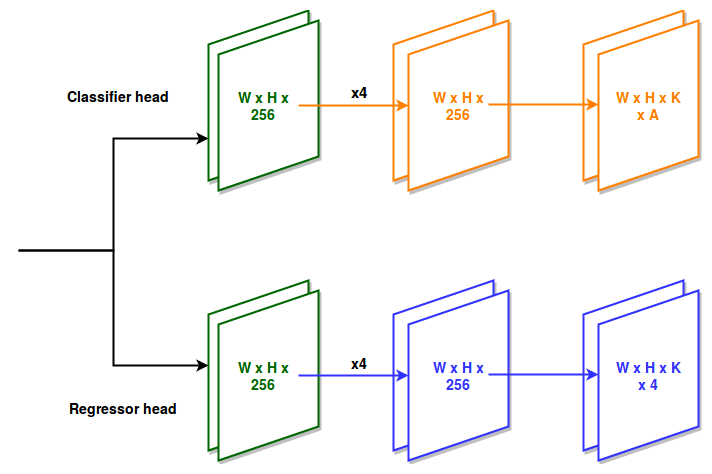
\includegraphics[width=0.95\textwidth]{subnets.png}
	\caption{Classifier and regressor head architectures}
	\label{fig:subnets}
\end{figure}

Output boxes are generated by taking positive foreground anchors and adding their box offsets to the corresponding coordinates. Overlapping boxes are merged using non-maximal supression.

Both the classifier and regressor heads are shared among all layer feature maps. The authors in \cite{Lin_2017_fpn} found that using different heads for each layer only showed marginal improvements. This implies that even at different levels of embedding, the learned features are similar enough for a single classifier/regressor to learn from.

In \cite{Lin_2017_fpn}, the authors also applied FPN to Faster R-CNN, a two-stage detector, where it functions as the region proposal network. Each target region is mapped to a single feature level, determined by its size. Larger ROIs are put into finer feature maps.

\subsection{Focal Loss}
RetinaNet employs the same bottom-up to top-down architecture as FPN. The primary improvement in RetinaNet is a novel loss function called Focal Loss. Focal Loss builds upon Balanced Cross Entropy, a modified version of the Cross Entropy function used to handle large class imbalances:
\begin{equation}
    CE(p_t) = -\alpha_t log(p_t)
\end{equation}
where $\alpha_t$ is a weighting factor determining how much to "focus" on negative examples as opposed to positives. In essence, $\alpha_t$ controls which class is prioritized during the training process. Focal Loss goes one step further and seeks to control how much to prioritize "hard" examples:
\begin{equation}
    FL(p_t) = -\alpha_t(1- p_t)^\gamma log(p_t)
\end{equation}
where $\gamma$ is the focusing parameter. We can see that by adding the modulating factor $-(1- p_t)^\gamma$, an example's loss diminishes as the model's prediction approaches the ground truth. In other words, \textit{easier} examples are down-weighted, therefore allowing models to focus on hard examples. As $\gamma$ increases, the model focuses more on harder examples. This transition is smooth, as seen in Figure \ref{fig:focal_loss}.

\begin{figure}[htp]
	\centering
	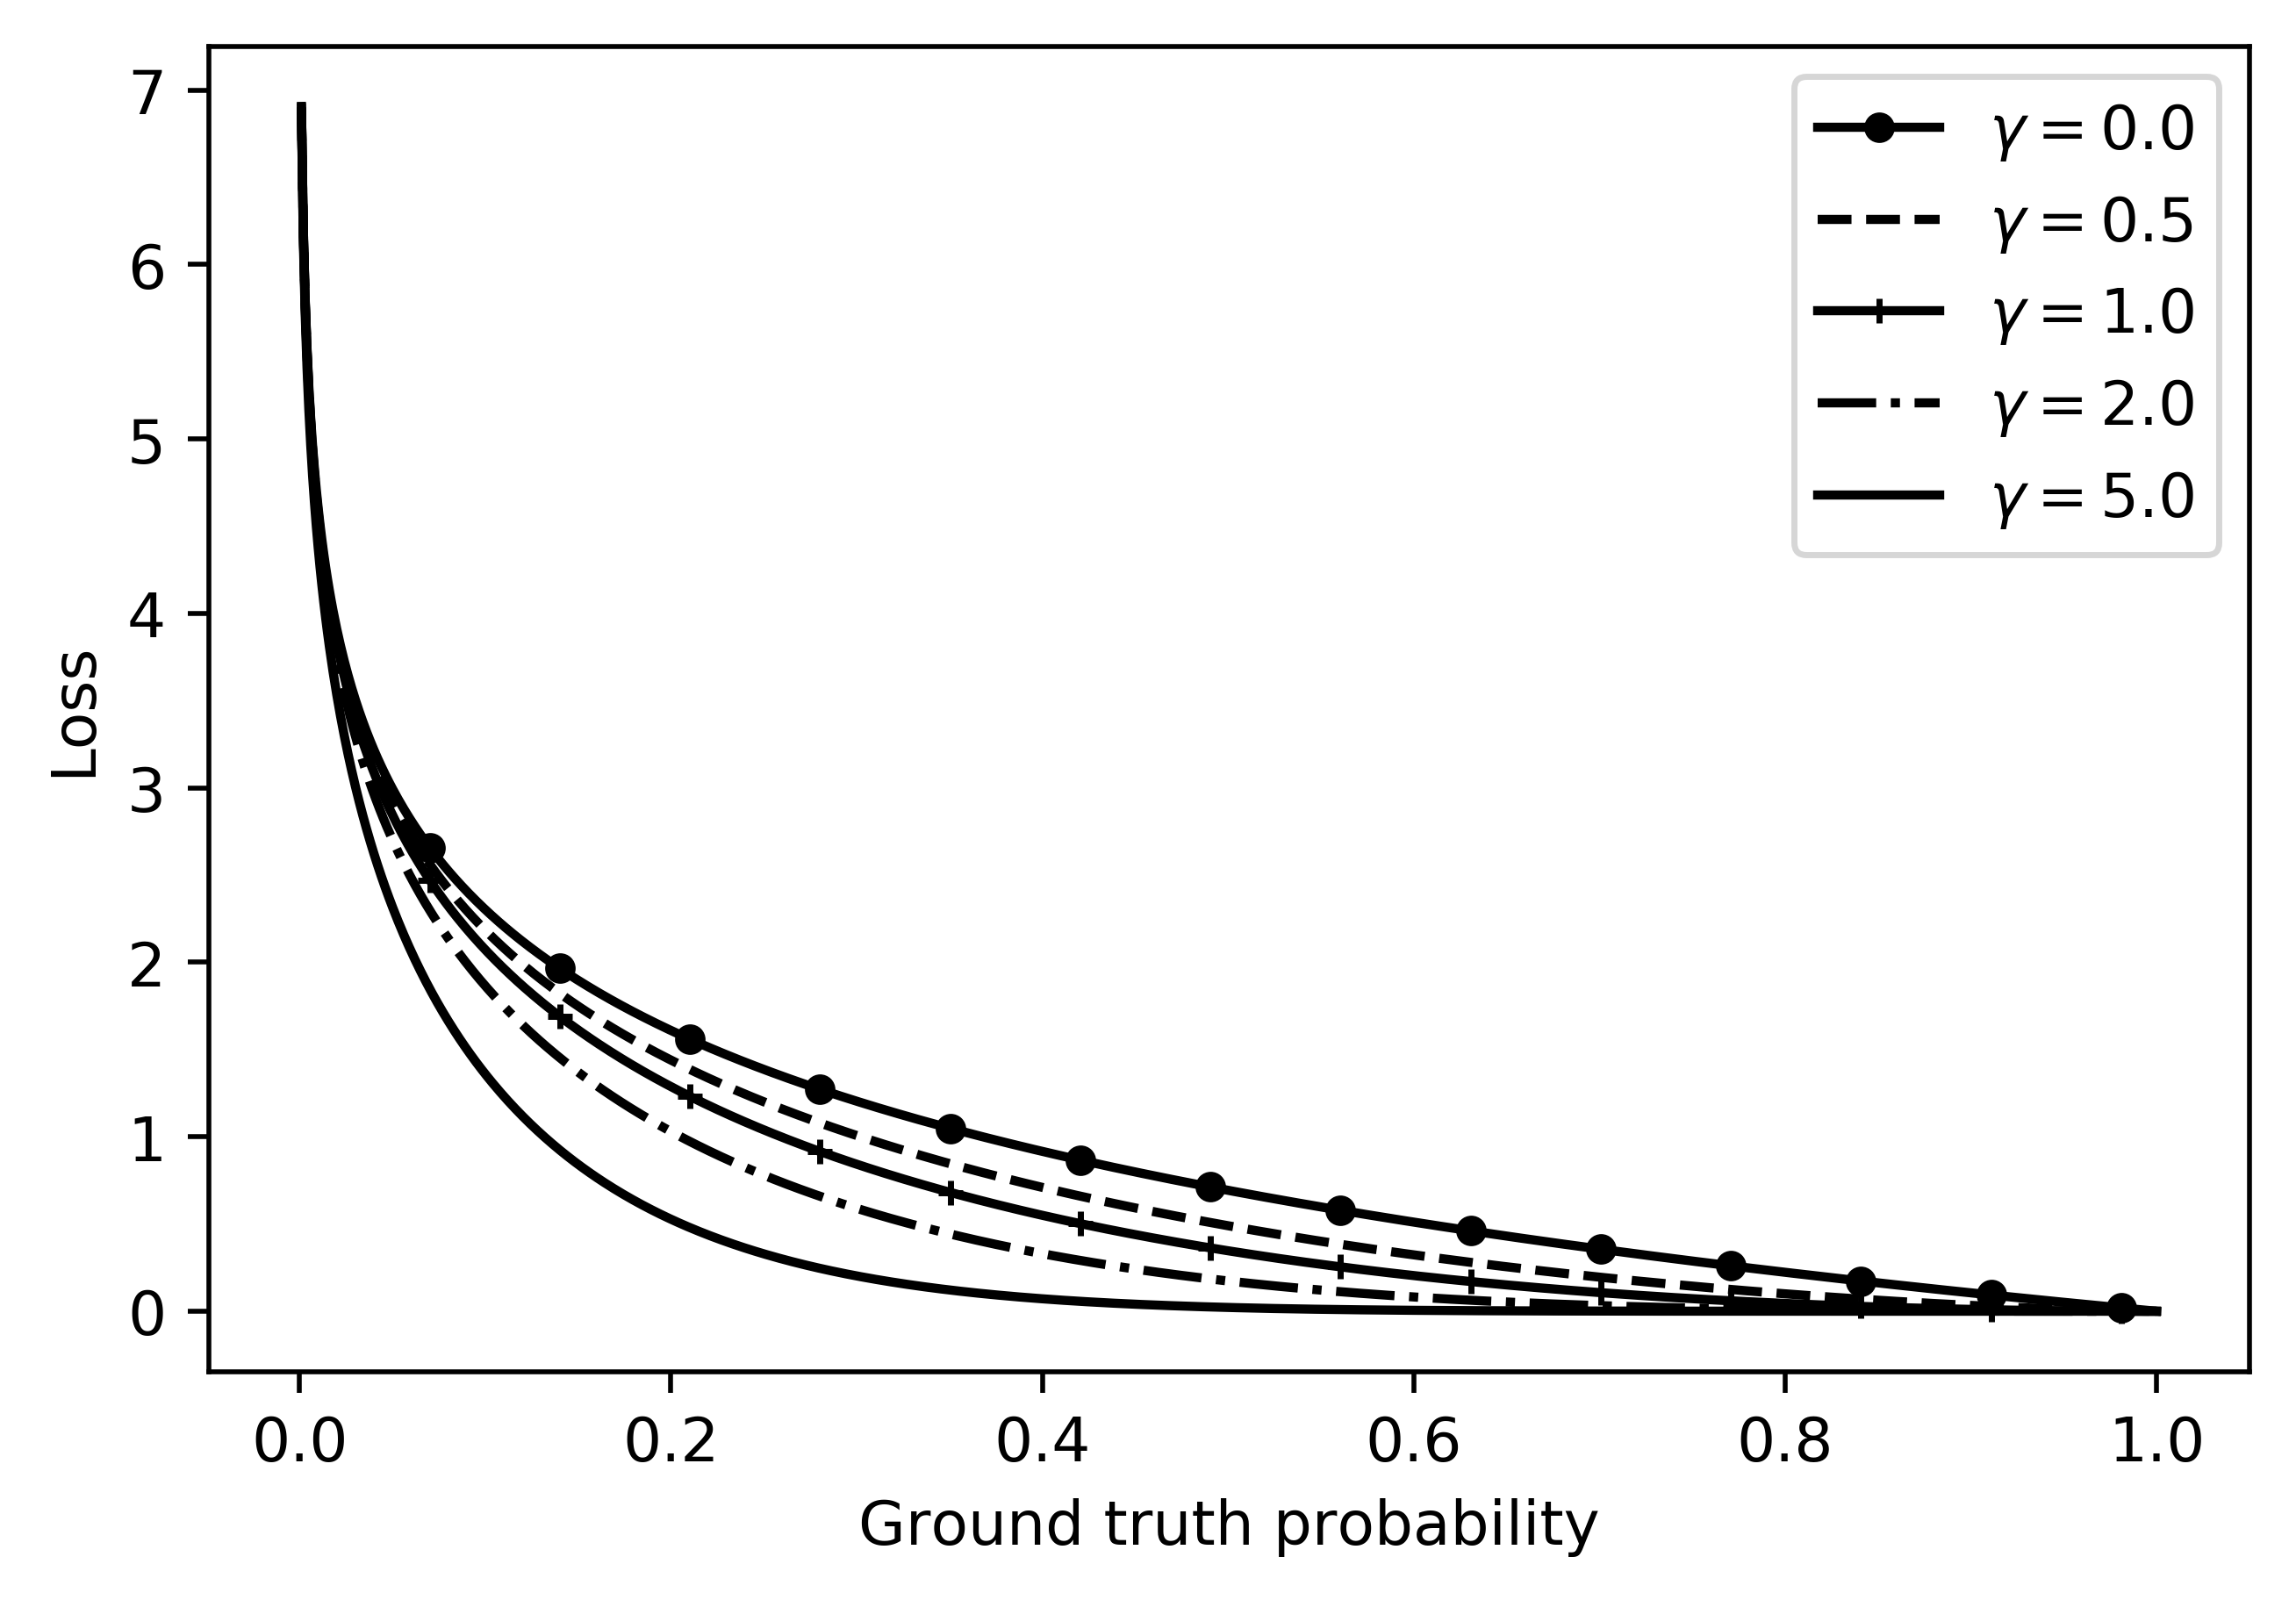
\includegraphics[width=0.7\textwidth]{focal_loss.png}
	\caption{Focal Loss values over ground truth probability for different values of $\gamma$}
	\label{fig:focal_loss}
\end{figure}

Aside from Focal Loss, RetinaNet makes several minor adjustments to FPN. Different anchor scales are used at each layer for denser anchor coverage. IoU thresholds when assigning anchor labels are also relaxed, with a positive threshold of 0.5 and negative threshold of 0.4.

RetinaNet was shown to achieve better results on the COCO dataset \cite{lin2014microsoft} than Faster-RCNN, while also being faster.

When applied to the text detection problem, we take special note of the anchors. Unlike regular objects, which often has a ratio from 1:2 to 2:1, text blocks are usually wide. Therefore, the anchors used on COCO in \cite{Lin_2017} would not perform well on this problem. Instead, we add wider ratios of 1:8, 1:6 and 1:4, which better fit our data.
